\chapter*{Bodové, algebraické a geometrické operace s obrazy}

V~praxi se často uplatňují operace, při nichž se modifikuje jas (případně intenzita barevných složek) tak, že jas výsledného obrazu v~každém bodě je nějakou funkcí jasu původního obrazu v~témže bodě. Takové operace nazýváme operacemi bodovými. Do operací algebraických vstupují zpravidla dva obrazy. Výsledný obraz se získává tak, že se jasy ve stejnolehlých bodech vstupních obrazů sčítají, odčítají, násobí nebo dělí. Na rozdíl od bodových a algebraických operací mění operace geometrické tvar a rozměry obrazu. O uvedených třídách operací pojednáme v této kapitole podrobněji. 

\section*{Bodové operace}

Nechť \textit{f}(\textit{x},\textit{y}) je obrazová funkce (jasová funkce) popisující vstupní obraz a \textit{g}(\textit{x},\textit{y}) obrazová funkce popisující obraz výstupní. Bodovou operací rozumíme transformaci obrazu podle předpisu

\begin{equation} \label{eq:6_1}
    g(x, y) = \varphi \left[ f \left( x, y \right) \right].
\end{equation}

Ze vztahu \eqref{eq:6_1} je zřejmé, že bodové operace vytvářejí výstupní obraz tak, že bodu o souřadnicích (\textit{x},\textit{y}) přiřadí hodnotu jasu, která je nějakou funkcí $\varphi$ jasu vstupního obrazu v bodě o stejných souřadnicích. Důvody pro provádění bodových transformací mohou být rozmanité. Uveďme několik příkladů: Citlivost prvků, které se při snímání obrazu používají často není lineární. Při fotometrické kalibraci kompenzujeme  bodovou operací nelinearitu snímacího prvku. Podobná je i situace na výstupu řetězce zpracovávajícího obraz, kde bodovou operací můžeme kompenzovat nelinearitu displeje. V~systémech pro zpracování obrazu je jednou z~nejpoužívanějších operací bodová operace provádějící změnu rozsahu nebo průběhu jasu.

\begin{figure}[th]
    \begin{center}
        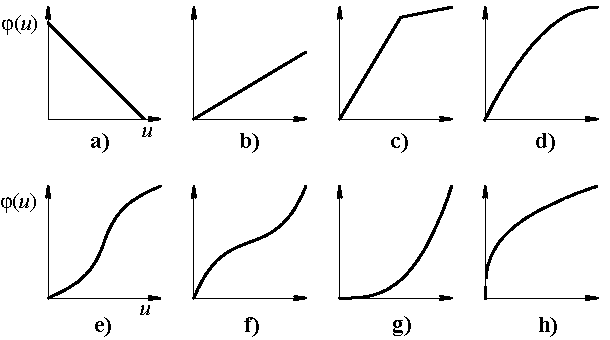
\includegraphics[scale=1.0]{06_bodoveoperace/images/img_6_1.pdf}
    \end{center}
    \caption{Příklady funkcí realizujících bodové operace: a), b) lineární funkce dle vztahu \eqref{eq:6_3}, c) funkce po částech lineární, d) kvadratická parabola \eqref{eq:6_4} ($c=1$), e), f) kubická parabola \eqref{eq:6_5}, g), h) exponencíální funkce \eqref{eq:6_6} ($\gamma = 3$, $\gamma = 1/3$).}
    \label{img:6_1}
\end{figure}

Předpokládáme, že jas (označme jej \textit{u}) vstupního obrazu může nabývat hodnot z intervalu $\langle$\textit{u}$_{\min}$, \textit{u}$_{\max}$ $\rangle$ a požadujeme, aby hodnoty \textit{u}$_{\min}$, \textit{u}$_{\max}$ byly transformovány na hodnoty \textit{v}$_1$=$\varphi$(\textit{u}$_{\min}$), \textit{v}$_2$=$\varphi$(\textit{u}$_{\max}$), které považujeme za známé. Zaveďme hodnotu $\xi$ vztahem

\begin{equation} \label{eq:6_2}
    \xi = \frac{u - u_{\min}}{u_{\max} - u_{\min}}.
\end{equation}

Jako příklady funkcí $\varphi(\xi)$ realizujících bodovou transformaci lze uvést např. následující funkce:

\begin{equation} \label{eq:6_3}
    \varphi(\xi) = v_1 + \xi ( v_2 - v_1 ),
\end{equation}

\begin{equation} \label{eq:6_4}
    \varphi(\xi) = v_1 + \left[ \xi + c \xi ( 1 - \xi ) \right] ( v_2 - v_1 ),
\end{equation}

\begin{equation} \label{eq:6_5}
    \varphi(\xi) = (1 - 3\xi^2 + 2\xi^3)v_1 + ( \xi -2\xi^2 + \xi^3)v_1' + (3\xi^2 - 2\xi^3)v_2 + ( -\xi^2 + \xi^3)v_2,
\end{equation}

\begin{equation} \label{eq:6_6}
    \varphi(\xi) = v_1 + \xi^\gamma (v_2 - v_1 ).
\end{equation}
kde $v_1' = \varphi'(u) |_{u=u_{\min}}$, $v_2' = \varphi'(u) |_{u=u_{\max}}$ a \textit{c},$\gamma$ jsou konstanty zvolené tak, aby bylo dosaženo žádaného průběhu funkce $\varphi$. Příklady průběhů funkcí jsou uvedeny na obr \ref{img:6_1}.

\subsection*{Vliv bodových operací na histogram jasu}

Nejprve uvedeme obecné úvahy týkající se histogramu jasu. Uvažujme diskrétní obrazy s jasem popsaným celými čísly. Obraz je definován nad oblastí sestávající z \textit{N} bodů. Nechť \textit{Nz} označuje počet bodů, jejichž jas je právě \textit{z}. Pro histogram (označme jej \textit{H}) jasu pak máme \textit{H}(\textit{z})=\textit{Nz}. Probírejme postupně jednotlivé body obrazu a vyšetřujme jejich jas. Na hodnotu jasu můžeme pohlížet jako na náhodnou proměnnou (označme ji \textbf{b}). Hodnota \textit{p}(\textit{z}) = \textit{H}(\textit{z})/\textit{N} = \textit{Nz}/\textit{N} udává pravděpodobnost jevu, že jas bodu je právě \textit{z}. Je zřejmé, že \textit{H}(\textit{z}) = \textit{Np}(\textit{z}). Poznamenejme, že pro hodnotu \textit{p}(\textit{z}) bývá též někdy používáno názvu normalizovaný histogram. Pro teoretické úvahy je výhodné zavést odpovídající pojem také pro spojité obrazy s reálnými hodnotami jasu. Nechť $\mathscr{P}$\{\textit{z}$<$\textbf{b}$\leq$\textit{z}+$\Delta$\textit{z}\} označuje pravděpodobnost jevu, že jas bodu nabývá hodnoty z intervalu (\textit{z},\textit{z}+$\Delta$\textit{z}$\rangle$, $\mathscr{S}$ nechť je plocha celého obrazu a $\mathscr{S}$\{\textit{z}$<$\textbf{b}$\leq$\textit{z}+$\Delta$\textit{z}\} nechť je plocha těch jeho částí, kde jas nabývá hodnoty z intervalu  (\textit{z},\textit{z}+$\Delta$\textit{z}$\rangle$. Ve spojitém případě má \textit{p}(\textit{z}) význam hustoty pravděpodobnosti

\begin{equation} \label{eq:6_7}
    p(z) = \lim\limits_{\Delta x \rightarrow 0} \frac{\mathscr{P} \left\{ z < \mathbf{b} \leq z+\Delta z \right\} }{\Delta z} = \lim\limits_{\Delta x \rightarrow 0} \frac{\mathscr{S} \left\{ z < \mathbf{b} \leq z+\Delta z \right\} }{\mathscr{S}\Delta z}
\end{equation}

\begin{figure}[th]
    \begin{center}
        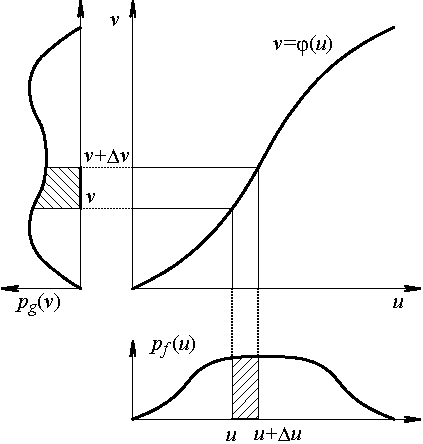
\includegraphics[scale=1.0]{06_bodoveoperace/images/img_6_2.pdf}
    \end{center}
    \caption{Vliv bodových operací na histogram obrazu.}
    \label{img:6_2}
\end{figure}

Vyšetřujme nyní, jak se histogram jasu mění vlivem bodových operací. Uvažujme spojité obrazy s~reálnými hodnotami jasu. Předpokládejme, že hustota pravděpodobnosti jasu vstupního obrazu \textit{f} je známa (označme ji \textit{p}$_f$) a že na obraz \textit{f} byla aplikována bodová operace popsaná rovnicí \eqref{eq:6_1}. Ukážeme, jak lze stanovit hustotu pravděpodobnosti jasu výstupního obrazu \textit{g} (označme ji \textit{p}$_g$). Nechť \textit{u},\textit{v} značí vstupní resp. výstupní jas. Je tedy \textit{v}=$\varphi$(\textit{u}). Předpokládejme, že $\varphi$ je bijekcí, a že lze proto konstruovat inverzní funkci \textit{u}=$\varphi^{-1}$(\textit{v}). Uvažujme interval $\langle$\textit{u}, \textit{u}+$\Delta$\textit{u}$\rangle$ vstupních jasů. Tomuto intervalu odpovídá interval $\langle$\textit{v},\textit{v}+$\Delta$\textit{v}$\rangle$ = $\langle$$\varphi$(\textit{u}), $\varphi$(\textit{u}+$\Delta$\textit{u})$\rangle$ jasů výstupních (obr. \ref{img:6_2}). Řekněme, že ve vstupním obraze měla jistá plocha obrazu jas z intervalu $\langle$\textit{u},\textit{u}+$\Delta$\textit{u}$\rangle$. Po transformaci bude mít tatáž plocha  jas z intervalu $\langle$\textit{v},\textit{v}+$\Delta$\textit{v}$\rangle$. Vzhledem ke vztahu \eqref{eq:6_7} proto máme 

\begin{equation} \label{eq:6_8}
    \int\limits_{v}^{v+\Delta v} p_g(z)\,dz = \int\limits_{u}^{u+\Delta u} p_f(z)\,dz.
\end{equation}

Jestliže jsou hodnoty $\Delta$\textit{u}, $\Delta$\textit{v} dostatečně malé, pak můžeme na základě vztahu \eqref{eq:6_8} také psát

\begin{equation} \label{eq:6_9}
    p_g(v)\Delta v = p_f(u)\Delta u.
\end{equation}

Odtud získáme pro výpočet hustoty pravděpodobnosti \textit{p}$_g$(\textit{v}) předpis

\begin{equation} \label{eq:6_10}
    p_g(v) = \frac{p_f(u)}{\Delta v / \Delta u} = \frac{p_f(u)}{\varphi'(u)} = \frac{p_f [\varphi^{-1}(v)]}{\varphi'[\varphi^{-1}(v)]}.
\end{equation}

\noindent \textbf{Příklad 6.1.} Předpokládejme, že jasy vstupního obrazu jsou nezáporné (\textit{u}$\geq$0) a že hustota pravděpodobnosti jasu vstupního obrazu je popsána výrazem

\begin{equation}
    p_f(u) = \frac{2}{\sqrt{\pi}} \exp(-u^2). \nonumber
\end{equation}

\begin{figure}[th]
    \begin{center}
        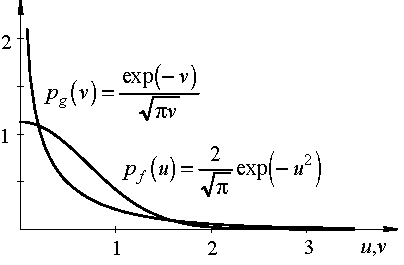
\includegraphics[scale=1.0]{06_bodoveoperace/images/img_6_3.pdf}
    \end{center}
    \caption{Hustoty pravděpodobností jasu z příkladu XXX.}
    \label{img:6_3}
\end{figure}

Výstupní obraz je definován vztahem

\begin{equation}
    g(x, y) = f^2(x, y). \nonumber
\end{equation}

Určíme hustotu pravděpodobnosti jasu výstupního obrazu. Máme \textit{v} = $\varphi$(\textit{u}) = \textit{u}$^2$, \textit{u} = $\varphi^{-1}$(\textit{v}) = $\surd$\textit{v}. Podle vztahu \eqref{eq:6_10} pak pro hledanou hustotu dostáváme

\begin{equation}
    p_g(v) = \frac{\exp(-v)}{\sqrt{\pi v}}. \nonumber
\end{equation}

\subsection*{Vyrovnání histogramu}

Vyrovnáním histogramu rozumíme provedení takové bodové operace, která zajistí rovnoměrné rozložení hustoty pravděpodobnosti jasu výsledného obrazu. Důvody k provedení operace mohou být následující: 1) Vyrovnání může vést ke zlepšení kvality obrazu subjektivně vnímané pozorovatelem. 2) Vyrovnání může být použito jako transformace zajišťující normalizované jednotné podmínky před dalším zpracováním obrazů (např. před segmentací a rozpoznáním). (Poznamenejme, že pro jistou třídu obrazů může však vyrovnání histogramu vést naopak i ke zhoršení subjektivně vnímané kvality. Jako příklad uvažte např. obraz vzniklý naskenováním výkresu obsahujícího černé čáry na bílém podkladě.) Zaměřme se nyní na problém stanovení funkce $\varphi$ ze vztahu \eqref{eq:6_1} tak, aby rozložení pravděpodobnosti \textit{p}$_g$ bylo rovnoměrné. Úvahy se zjednoduší, jestliže budeme předpokládat, že jas vstupního i výstupního obrazu je reprezentován reálnými čísly (obr. \ref{img:6_4}a). Z podmínky rovnoměrného rozložení hustoty pravděpodobnosti máme \textit{p}$_g$(\textit{v}) = 1/(\textit{v}$_{\max}$ $-$ \textit{v}$_{\min}$). Použitím vztahu \eqref{eq:6_10} pak dostaneme

\begin{equation} \label{eq:6_11}
    \varphi'(v) = \frac{p_f(u)}{p_g(v)} = p_f(u)(v_{\max} - v_{\min}).
\end{equation}

Odtud

\begin{equation} \label{eq:6_12}
    \varphi(u) = \int\limits_{u_{\min}}^{u} \varphi'(z)\,dz = (v_{\max} - v_{\min}) \int\limits_{u_{\min}}^{u} p_f(z)\,dz.
\end{equation}

\begin{figure}[th]
    \begin{center}
        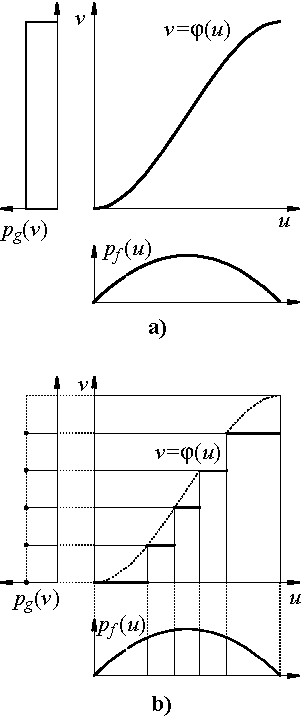
\includegraphics[scale=1.0]{06_bodoveoperace/images/img_6_4.pdf}
    \end{center}
    \caption{Vyrovnání histogramu jasu.}
    \label{img:6_4}
\end{figure}

Protože je podle předpokladu hustota \textit{p}$_f$(\textit{z}) známá, je vztah \eqref{eq:6_12} předpisem pro výpočet hledané funkce $\varphi$. Jestliže jsou jasy reprezentovány celými čísly, je zapotřebí několik dalších upřesnění. Zaměřme se nejprve na případ, kdy je celými čísly reprezentován pouze jas výstupního obrazu. Máme tedy \textit{v}$\in$\{\textit{v}$_{\min}$, \textit{v}$_{\min}$+1, \dots, \textit{v}$_{\max}$\}. Jasy vstupního obrazu jsou reálné. Funkce $\varphi$ má v tomto případě stupňovitý tvar (obr. \ref{img:6_4}b). Pro \textit{z}$\in$(\textit{u}$_v$,\textit{u}$_{v+1}$$\rangle$ platí $\varphi$(\textit{z}) = \textit{v}. Problémem je stanovit pro jednotlivé hodnoty \textit{v} odpovídající hodnoty \textit{u}$_v$. S přihlédnutím ke skutečnosti, že v tomto případě je \textit{p}$_g$(\textit{v}) = 1/(\textit{v}$_{\max}$ $-$ \textit{v}$_{\min}$ + 1), dostáváme z podmínky rovnoměrného rozdělení pravděpodobností pro hodnotu \textit{u}$_v$ (\textit{v}$_{\min}$ $\leq$\textit{v}$\leq$\textit{v}$_{\max}$) následující rovnici

\begin{equation} \label{eq:6_13}
    \frac{v - v_{\min}}{(v_{\max} - v_{\min} + 1)} = \int\limits_{u_{\min}}^{u_v} p_f(z)\,dz.
\end{equation}

\noindent Jestliže je celými čísly reprezentován jas jak výstupního tak i vstupního obrazu, pak je funkce $\varphi$ diskrétní. Stejně jako v předchozím případě, je i zde problémem stanovit pro jednotlivé hodnoty \textit{v} odpovídající hodnoty \textit{u}$_v$. Hledanou hodnotu \textit{u}$_v$ lze určit jako nejmenší hodnotu, pro kterou je splněna nerovnost

\begin{equation} \label{eq:6_14}
    \frac{v - v_{\min}}{(v_{\max} - v_{\min} + 1)} = \sum\limits_{z=u_{\min}}^{u_v} p_f(z).
\end{equation}

Jak z uvedeného postupu vyplývá, nelze v případě, kdy je celými čísly reprezentován jas výstupního i vstupního obrazu, dosáhnout vyrovnání histogramu zcela přesně. Histogram je vyrovnán pouze přibližně.

\section*{Algebraické operace s obrazy}

Nechť \textit{f}$_1$(\textit{x},\textit{y}), \textit{f}$_2$(\textit{x},\textit{y}) jsou známé obrazy. Algebraickou operací rozumíme postup, kdy je výsledný obraz \textit{g}(\textit{x},\textit{y}) získáván pomocí některého z~následujících vztahů:

\begin{equation} \label{eq:6_15}
    g(x, y) = f_1(x, y) + f_2(x, y),
\end{equation}

\begin{equation} \label{eq:6_16}
    g(x, y) = f_1(x, y) - f_2(x, y),
\end{equation}

\begin{equation} \label{eq:6_17}
    g(x, y) = f_1(x, y) \times f_2(x, y),
\end{equation}

\begin{equation} \label{eq:6_18}
    g(x, y) = f_1(x, y) \div f_2(x, y).
\end{equation}

Uveďme několik příkladů, kdy mohou být algebraické operace použity v~praxi: Při snímání kamerou je někdy vlivem nedokonalosti objektivu obrázek uprostřed světlejší a na krajích (nejvíce v~rozích) tmavší. Uvedenou vadu objektivu můžeme považovat za multiplikativní chybu a korigovat ji pomocí vztahů \eqref{eq:6_17} nebo \eqref{eq:6_18}. Obraz \textit{f}$_1$ je obraz, který má být korigován. Korekční hodnoty obsažené v obrazu \textit{f}$_2$ snadno vypočítáme např. z hodnot získaných sejmutím bílé rovnoměrně osvětlené plochy. Podobně lze korigovat systematickou chybu vznikající nerovnoměrným osvětlením předlohy při snímání kamerou. Při snímání scény, v~níž se pohybují objekty, lze rozdílu po sobě jdoucích obrazů využít k~detekci pohybu. Použití sčítání obrazu pro redukci šumu ukážeme podrobněji v~samostatné podkapitole.

\subsection*{Vliv algebraických operací na histogram jasu}

Nechť \textit{p}$_1$(\textit{z}), \textit{p}$_2$(\textit{z}) jsou hustoty pravděpodobnosti jasu v obrazech \textit{f}$_1$(\textit{x},\textit{y}), \textit{f}$_2$(\textit{x},\textit{y}). Stanovíme hustotu pravděpodobnosti \textit{p}(\textit{z}) jasu obrazu \textit{g}(\textit{x},\textit{y}) vzniklého součtem dle vztahu \eqref{eq:6_15}. Označme \textit{p}$_{1,2}$(\textit{u},\textit{v}) sdruženou hustotu pravděpodobnosti jasu v prvním a druhém obraze. Předpokládáme, že vstupní    obrazy jsou nezávislé, a že proto platí \textit{p}$_{1,2}$(\textit{u},\textit{v}) = \textit{p}$_1$(\textit{u})\textit{p}$_2$(\textit{v}). Podle vztahu \eqref{eq:6_15} je hodnoty \textit{z} jasu v obraze \textit{g}(\textit{x},\textit{y}) dosaženo tehdy, jestliže při jasu \textit{v} v obraze \textit{f}$_2$ je jas v obraze \textit{f}$_1$ roven hodnotě \textit{u}=\textit{z}$-$\textit{v}. Odtud vychází pro hledanou hustotu \textit{p}(\textit{z}) vztah 

\begin{equation} \label{eq:6_19}
    p(z) = \int\limits_{-\infty}^{\infty}p_{1,2}(z - v, v)\,dv = \int\limits_{-\infty}^{\infty}p_1(z-v)p_2(v)\,dv = p_1(z) \ast p_2(z).
\end{equation}

Vztah \eqref{eq:6_19} ukazuje, že hustota pravděpodobnosti jasu výsledného obrazu je rovna konvoluci hustot pravděpodobností jasů obou obrazů vstupních. Získaný výsledek lze snadno rozšířit také na rozdíl  obrazů dle vztahu \eqref{eq:6_16}. Postačí položit $\tilde{f}_2(x, y) = -f_2(x, y)$, čímž převedeme rozdíl na součet. Pro hustotu pravděpodobnosti jasu obrazu $\tilde{f}_2$ máme $\tilde{p}_2(z) = p_2(-z)$.

\subsection*{Využití průměrování k redukci šumu}

V tomto odstavci podrobněji popíšeme jednu z praktických aplikací sčítání obrazů. Nechť \textit{f}(\textit{x},\textit{y}) je teoretický obraz neměnný v čase. Při snímání získáváme ovšem obraz, který je poškozen šumem. Obraz proto snímáme opakovaně \textit{M}-krát. Při \textit{i}-tém sejmutí obdržíme obraz \textit{f}(\textit{x},\textit{y})+\textit{ni}(\textit{x},\textit{y}), kde \textit{n}$_i$ je šum. Za aproximaci teoretického obrazu můžeme intuitivně brát průměr

\begin{equation} \label{eq:6_20}
    \tilde{f}(x, y) = \frac{1}{M} \sum\limits_{i=1}^{M} [ f(x, y) + n_i(x, y) ].
\end{equation}

Ukážeme, že použití průměru podle rovnice \eqref{eq:6_20} objektivně vede ke zlepšení kvality sejmutého   obrazu. K hodnocení kvality použijeme poměru signál-šum, který je definován vztahem

\begin{equation} \label{eq:6_21}
    SNR(x, y) = \frac{f(x, y)}{\sqrt{\mathrm{E}\left\{ n^2(x, y) \right\}}}
\end{equation}

Pro hodnotu poměru signál-šum v obraze vzniklém průměrováním \textit{M} obrazů odtud vychází

\begin{equation} \label{eq:6_22}
    SNR_M(x, y) = \frac{f(x, y)}{\sqrt{\mathrm{E}\left\{ \left[ \frac{1}{M} \sum\limits_{i=1}^{M} n_i(x, y) \right]^2 \right\}}}
\end{equation}

Výraz \eqref{eq:6_22} dále upravíme. Při tom využijeme následujících předpokladů: 1) \textit{n}$_i$(\textit{x},\textit{y}) je náhodná proměnná, pro niž platí $\mathrm{E}$\{\textit{n}$_i$(\textit{x},\textit{y})\}=0; 2) náhodné proměnné \textit{n}$_i$(\textit{x},\textit{y}), \textit{n}$_j$(\textit{x},\textit{y}) jsou nekorelované, a proto platí $\mathrm{E}$\{\textit{n}$_i$(\textit{x},\textit{y}) \textit{n}$_j$(\textit{x},\textit{y})\} = $\mathrm{E}$\{\textit{n}$_i$(\textit{x},\textit{y})\}$\mathrm{E}$\{\textit{n}$_j$(\textit{x},\textit{y})\}; 3) $\mathrm{E}$\{\textit{n}$_i^2$(\textit{x},\textit{y})\} = $\mathrm{E}$\{\textit{n}$_j^2$(\textit{x},\textit{y})\} = $\mathrm{E}$\{\textit{n}$^2$(\textit{x},\textit{y})\}. Postupně dostáváme

\begin{equation} \label{eq:6_23} 
    SNR_{M} \left(x, y\right) = \frac{Mf\left(x, y\right)}{\sqrt{\mathrm{E}\left\{\sum\limits_{i=1}^{M}n_{i}^{2} \left(x,y\right) \right\}} } = \sqrt{M} \frac{f(x, y)}{\sqrt{\mathrm{E}\{n^2(x, y)\}}} = \sqrt{M} SNR(x, y).
\end{equation}

Vztah \eqref{eq:6_23} ukazuje, že průměrováním z \textit{M} obrazů se poměr signál-šum zvětšil $\surd$\textit{M}-krát.

\section*{Geometrické transformace obrazu}

Geometrické transformace mění tvar nebo rozměry obrazu. Obecně jsou popsány vztahem

\begin{equation} \label{eq:6_24} 
    g\left(x,y\right)=f\left[\varphi \left(x,y\right),\psi \left(x,y\right)\right].  
\end{equation}

Je zřejmé, že geometrická transformace je zcela zadána funkcemi $\varphi$(\textit{x},\textit{y}), $\psi$(\textit{x},\textit{y}). Vztah \eqref{eq:6_24} navíc podává i praktický návod na to, jak transformaci provést. Předpokládejme, že obrazy \textit{f}(\textit{x},\textit{y}) i \textit{g}(\textit{x},\textit{y}) jsou diskrétní. Na základě vztahu \eqref{eq:6_24} lze postupně probírat všechny body výstupního obrazu \textit{g} a pro každý bod (\textit{x},\textit{y}) určit odpovídající polohu [$\varphi$(\textit{x},\textit{y}), $\psi$(\textit{x},\textit{y})] ve vstupním obraze \textit{f}. Hodnota jasu \textit{f}[$\varphi$(\textit{x},\textit{y}), $\psi$(\textit{x},\textit{y})] je pak vzata jako hodnota \textit{g}(\textit{x},\textit{y}). Zatímco \textit{x},\textit{y} nabývají celočíselných hodnot (postupujeme po celočíselných souřadnicích pixelů výstupního obrazu), jsou hodnoty $\varphi$(\textit{x},\textit{y}), $\psi$(\textit{x},\textit{y}) obvykle reálné, nikoli celočíselné. Podle předpokladu je však i vstupní obraz \textit{f} diskrétní, a proto i pro něj jsou hodnoty jasu známy jen v bodech o celočíselných souřadnicích. Pro získání hodnot v mezilehlých bodech o neceločíselných souřadnicích lze využít metod, které byly podrobněji popsány v~podkapitole \ref{sec:prakticke_metody_rekonstrukce_obrazu}. V praxi se nejčastěji používá bilineární interpolace nebo interpolace vyššího řádu.    

Zabývejme se nyní podrobněji funkcemi $\varphi$(\textit{x},\textit{y}), $\psi$(\textit{x},\textit{y}). Nejobecnějším požadavkem je, aby dvojice [$\varphi$(\textit{x},\textit{y}), $\psi$(\textit{x},\textit{y})] byla homeomorfismem (nesplnění tohoto požadavku by způsobilo „roztrhání`` obrazu). Kromě toho bývají obvykle požadovány i jiné vlastnosti. Jsou-li funkce $\varphi$(\textit{x},\textit{y}), $\psi$(\textit{x},\textit{y}) lineární, pak je transformace \eqref{eq:6_24}  transformací afinní. Afinní transformace je zadána šesti hodnotami \textit{a}$_{11}$, \textit{a}$_{12}$, \textit{a}$_{21}$, \textit{a}$_{22}$, \textit{b}$_1$, \textit{b}$_2$ a lze ji zapsat následujícím vztahem

\begin{equation} \label{eq:6_25}
    \left[\begin{array}{c} {\varphi \left(x,y\right)} \\ {\psi \left(x,y\right)} \end{array}\right]=\left[\begin{array}{cc} {a_{11} } & {a_{12} } \\ {a_{21} } & {a_{22} } \end{array}\right]\left[\begin{array}{c} {x} \\ {y} \end{array}\right]+\left[\begin{array}{c} {b_{1} } \\ {b_{2} } \end{array}\right].  
\end{equation}

\noindent \textbf{Příklad 6.2.} Uvažujme diskrétní obraz rozměru \textit{M}$\times$\textit{N} bodů popsaný obrazovou funkcí \textit{f}(\textit{m},\textit{n}) (obr. \ref{img:6_5}). Provedeme rotaci obrazu kolem levého dolního rohu o úhel $\varphi$ (0$\leq$$\alpha$$\leq$$\pi$/2). Rozměry obrazu vzniklého rotací budou $\lceil$(\textit{N}$-$1)$\sin$ $\varphi$ + (\textit{M}$-$1)$\cos$ $\varphi$ + 1$\rceil$ $\times \lceil$ (\textit{N}$-$1)cos $\varphi$ + (\textit{M}$-$1) sin $\varphi$ + 1 $\rceil$ bodů. Počátek (0,0) předpokládáme u obou obrazů v levém dolním rohu. Označne $\tilde{x},\tilde{y}$ souřadnice v původním a \textit{x},\textit{y} souřadnice v novém obraze. Pro transformaci souřadnic z původního do nového obrazu snadno získáme předpis

\begin{equation}
    x = \tilde{x}\cos \varphi -\tilde{y}\sin \varphi +(N-1) \sin \varphi, \nonumber
\end{equation}

\begin{equation}
    y = \tilde{x}\sin \varphi +\tilde{y}\cos \varphi. \nonumber 
\end{equation}

Odtud máme

\begin{equation}
    \left[\begin{array}{c} {\varphi \left(x,y\right)} \\ {\psi \left(x,y\right)} \end{array}\right]=\left[\begin{array}{c} {\tilde{x}} \\ {\tilde{y}} \end{array}\right]=\left[\begin{array}{cc} {\cos \varphi } & {\sin \varphi } \\ {-\sin \varphi } & {\cos \varphi } \end{array}\right]\left[\begin{array}{c} {x} \\ {y} \end{array}\right]+\left(N-1\right)\left[\begin{array}{c} {-\sin \varphi \cos \varphi } \\ {\sin ^{2} \varphi } \end{array}\right]. \nonumber
\end{equation}

Prakticky provedeme transformaci tak, že probíráme všechny body výstupního obrazu jeden po druhém. Poloha bodu ve výstupním obraze je specifikována celočíselnou dvojicí \textit{x},\textit{y}. Jestliže platí [0$\leq$$\varphi$(\textit{x},\textit{y})$\leq$\textit{M}$-$1]\&[0$\leq$$\psi$(\textit{x},\textit{y})$\leq$\textit{N}$-$1], určíme hodnotu \textit{g}(\textit{x},\textit{y}) jako hodnotu \textit{f}[$\varphi$(\textit{x},\textit{y}), $\psi$(\textit{x},\textit{y})], kterou vypočítáme interpolací. V opačném případě položíme např. \textit{g}(\textit{x},\textit{y})=0.

\begin{figure}[th]
    \begin{center}
        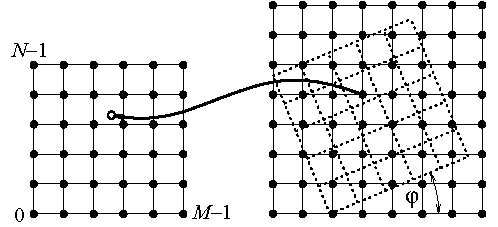
\includegraphics[scale=1.0]{06_bodoveoperace/images/img_6_5.pdf}
    \end{center}
    \caption{Afinní transformace obrazu - rotace.}
    \label{img:6_5}
\end{figure}

\noindent \textbf{Příklad 6.3.} Geometrickou transformací, která se v praxi uplatňuje velmi často, je změna rozměru obrazu. Opět uvažujme diskrétní obraz rozměru \textit{M}$\times$\textit{N} bodů. Tento obraz má být transformován tak, aby rozměry výstupního obrazu byly \textit{P}$\times$\textit{Q}. Snadno obdržíme vztah

\begin{equation}
    \left[\begin{array}{c} {\varphi \left(x,y\right)} \\ {\psi \left(x,y\right)} \end{array}\right]=\left[\begin{array}{cc} {\frac{P-1}{M-1} } & {0} \\ {0} & {\frac{Q-1}{N-1} } \end{array}\right]\left[\begin{array}{c} {x} \\ {y} \end{array}\right].\nonumber
\end{equation}

Obecnější než transformace afinní jsou transformace projektivní. Jak afinní tak projektivní transformace zachovávají linearitu transformovaných útvarů (přímky se transformují opět na přímky). Na rozdíl od afinních transformací však projektivní transformace nezachovávají rovnoběžnost. Projektivní transformace se uplatňují zejména v případech, které nějakým způsobem souvisí se středovým promítáním. Příkladem praktické úlohy je transformace, při níž má být obraz deformován tak, aby budil dojem, že je umístěn na nějaké obecně umístěné rovině v prostoru, kterou zobrazujeme středovým promítáním.

Při popisu projektivních transformací se zpravidla používá homogenních souřadnic. Homogenní souřadnice reprezentují bod v \textit{n}-rozměrném afinním prostoru jako směr v jistém přidruženém (\textit{n}+1)-rozměrném vektorovém prostoru. Uvažujme dvojrozměrný afinní prostor a zaveďme přidružený trojrozměrný vektorový prostor a souřadnou soustavu v~něm tak, jak je znázorněno na obr. \ref{img:6_6}. V afinním prostoru uvažujme bod, jehož afinní souřadnice jsou (\textit{x},\textit{y}). Homogenními souřadnicemi uvažovaného bodu je trojice (\textit{wx},\textit{wy},\textit{w}), kde \textit{w} je libovolné reálné číslo \textit{w}$\neq$0. V homogenních souřadnicích je tedy každý bod reprezentován nekonečným počtem vektorů v přidruženém vektorovém prostoru, které jsou ovšem všechny navzájem kolineární. Speciálně můžeme také volit \textit{w}=1. Dostaneme tak trojici (\textit{x},\textit{y},1). Zvláštní význam této volby je patrný z obr. \ref{img:6_6}. Je-li naopak trojice (\textit{x},\textit{y},\textit{w}) homogenními souřadnicemi nějakého bodu, pak také trojice (\textit{x}/\textit{w},\textit{y}/\textit{w},1) je homogenními souřadnicemi téhož bodu a dvojice (\textit{x}/\textit{w},\textit{y}/\textit{w}) je jeho souřadnicemi afinními. Projektivní transformace bodu o afinních souřadnicích (\textit{x},\textit{y}) je popsána rovnicí

\begin{equation} \label{eq:6_26} 
    \left[\begin{array}{c} {\varphi \left(x,y\right)} \\ {\psi \left(x,y\right)} \\ {\omega \left(x,y\right)} \end{array}\right]=\left[\begin{array}{ccc} {p_{11} } & {p_{12} } & {p_{13} } \\ {p_{21} } & {p_{22} } & {p_{23} } \\ {p_{31} } & {p_{32} } & {p_{33} } \end{array}\right]\left[\begin{array}{c} {x} \\ {y} \\ {1} \end{array}\right].  
\end{equation} 

\begin{figure}[th]
    \begin{center}
        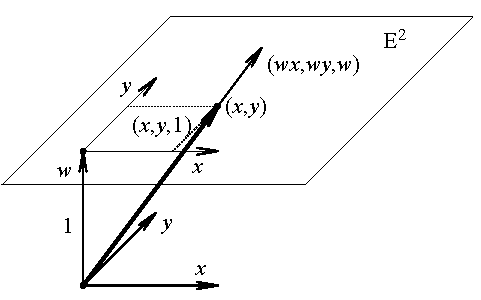
\includegraphics[scale=1.0]{06_bodoveoperace/images/img_6_6.pdf}
    \end{center}
    \caption{Zavedení homogenních souřadnic.}
    \label{img:6_6}
\end{figure}

Homogenní souřadnice bodu po transformaci jsou ($\varphi$(\textit{x},\textit{y}), $\psi$(\textit{x},\textit{y}), $\omega$(\textit{x},\textit{y})), odkud pro afinní souřadnice plyne vztah ($\varphi$(\textit{x},\textit{y})/$\omega$(\textit{x},\textit{y}), $\psi$(\textit{x},\textit{y})/ $\omega$(\textit{x},\textit{y})). Ze vztahu \eqref{eq:6_26} vyplývá, že ve dvojrozměrném prostoru je projektivní transformace je popsána devíti hodnotami \textit{p}$_{11}$, \textit{p}$_{12}$, \dots, \textit{p}$_{33}$. Uvedené hodnoty lze ovšem násobit libovolnou  nenulovou reálnou konstantou, aniž by se výsledek transformace změnil (násobením se sice změní délka vektoru na levé straně vztahu \eqref{eq:6_26}, ale bod, který je vektorem reprezentován, je stále tentýž).

\noindent \textbf{Příklad 6.4.} Uvažujme projektivní transformaci zadanou tak, že pro čtveřici bodů $\tilde{A}_{1} ,\tilde{A}_{2} ,\tilde{A}_{3} ,\tilde{A}_{4} $ ve vstupním obraze jsou předepsány jim odpovídající body $A_{1} ,A_{2} ,A_{3} ,A_{4} $ v obraze výstupním (na obr. \ref{img:6_7} jsou jako body $\tilde{A}_{1}, \tilde{A}_{2}, \tilde{A}_{3}, \tilde{A}_{4}$ zvoleny rohy obrazu). Naznačíme postup odvození transformační matice ze vztahu \eqref{eq:6_26}. Souřadnice bodu $\tilde{A}_{i}$ v původním obraze označíme $\tilde{x}_{i} ,\tilde{y}_{i} $. Poloha korespondujícího bodu \textit{A}$_i$ ve výstupním obraze je předepsána souřadnicemi $\tilde{x}_i$, $\tilde{y}_i$. Dále zavedeme označení \textbf{p}$_1$=(\textit{p}$_{11}$,\textit{p}$_{12}$,\textit{p}$_{13}$)$^\top$, \textbf{p}$_2$=(\textit{p}$_{21}$,\textit{p}$_{22}$,\textit{p}$_{23}$)$^\top$, \textbf{p}$_3$=(\textit{p}$_{31}$,\textit{p}$_{32}$,\textit{p}$_{33}$)$^\top$, \textbf{x}$_i$=(\textit{x}$_i$,\textit{y}$_i$,1)$^\top$. Na základě vztahu \eqref{eq:6_26} nyní pro každý ze zadaných bodů dostáváme 

\begin{equation}
    \left[\begin{array}{c} {\tilde{w}_{i} \tilde{x}_{i} } \\ {\tilde{w}_{i} \tilde{y}_{i} } \\ {\tilde{w}_{i} } \end{array}\right]=\left[\begin{array}{c} {p_{1}^\top} \\ {p_{2}^\top} \\ {p_{3}^\top} \end{array}\right]x_{i}. \nonumber
\end{equation}

Ze třetí rovnice v uvedeném vztahu máme $\tilde{w}_{i} =p_{3}^\top x_{i} $. Dosazením do prvních dvou rovnic po úpravě dostaneme

\begin{equation}
    \left[\begin{array}{ccc} {x_{i}^\top} & {0} & {-\tilde{x}_{i} x_{i}^\top} \\ {0} & {x_{i}^\top} & {-\tilde{y}_{i} x_{i}^\top} \end{array}\right]\left[\begin{array}{c} {p_{1} } \\ {p_{2} } \\ {p_{3} } \end{array}\right]=\left[\begin{array}{c} {0} \\ {0} \end{array}\right]. \nonumber
\end{equation}

Vidíme, že každý ze zadaných bodů přispívá k nalezení transformační matice dvěma rovnicemi, což dává celkem osm rovnic pro devět neznámých. Protože víme, že transformační matici je možné násobit libovolným reálným číslem, aniž by se výsledek transformace změnil, zvolíme k zajištění jednoznačnosti řešení doplňující podmínku. Nejsnáze se prakticky realizuje postup, kdy některý z prvků transformační matice položíme roven předem zvolené hodnotě (prosíme čtenáře, aby promyslel úskalí tohoto řešení).

\begin{figure}[th]
    \begin{center}
        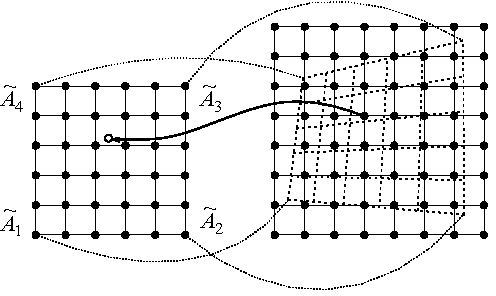
\includegraphics[scale=1.0]{06_bodoveoperace/images/img_6_7.pdf}
    \end{center}
    \caption{Projektivní transformace obrazu.}
    \label{img:6_7}
\end{figure}

Nelineární geometrickou transformací obrazu rozumíme transformaci, kde $\varphi$(\textit{x},\textit{y}), $\psi$(\textit{x},\textit{y}) jsou nelineární funkce. Nečastěji se jedná o polynomy. Můžeme je volit např. ve tvaru

\begin{equation} \label{eq:6_27}
    \varphi \left(x,y\right)=x+\Delta x\left(x,y\right), \quad \psi \left(x,y\right)=y+\Delta y\left(x,y\right),
\end{equation}
kde

\begin{equation} \label{eq:6_28}
    \Delta x\left(x,y\right)=\sum _{r=0}^{m}\sum _{s=0}^{m-r}a_{rs} x^{r} y^{s}, \quad \Delta y\left(x,y\right)=\sum _{r=0}^{m}\sum _{s=0}^{m-r}b_{rs} x^{r} y^{s}
\end{equation}
nebo také

\begin{equation} \label{eq:6_29}
    \Delta x\left(x,y\right)=\sum _{r=0}^{m}\sum _{s=0}^{m}a_{rs} x^{r} y^{s}, \quad \Delta y\left(x,y\right)=\sum _{r=0}^{m}\sum _{s=0}^{m}b_{rs} x^{r} y^{s}.
\end{equation}

Ze vztahu \eqref{eq:6_27} je zřejmé, že funkce $\Delta$\textit{x}(\textit{x},\textit{y}), $\Delta$\textit{y}(\textit{x},\textit{y}) popisují „přemístění`` bodu, ke kterému během transformace dojde. Zavedení funkcí $\Delta$\textit{x}(\textit{x},\textit{y}), $\Delta$\textit{y}(\textit{x},\textit{y}) je názorné a také výhodné pro praktickou implementaci. Polynomy, které se pro transformaci používají, v~praxi zpravidla nebývají příliš vysokého stupně (obvykle druhého nebo třetího). Neznámé hodnoty koeficientů \textit{a}$_{rs}$, \textit{b}$_{rs}$ je možné stanovit tak, že pro jistý počet bodů (\textit{x}$_i$,\textit{y}$_i$) předepíšeme hodnoty $\varphi$(\textit{x}$_i$,\textit{y}$_i$), $\psi$(\textit{x}$_i$,\textit{y}$_i$). To dává dvě soustavy rovnic

\begin{equation} \label{eq:6_30}
    \varphi \left(x_{i} ,y_{i} \right)=x_{i} +\sum_{r=0}^{m}\sum_{s=0}^{m-r}a_{rs} x_{i}^{r} y_{i}^{s},
    \quad
    \psi \left(x_{i} ,y_{i} \right)=y_{i} +\sum _{r=0}^{m}\sum _{s=0}^{m-r}b_{rs} x_{i}^{r} y_{i}^{s},
\end{equation} 
z~nichž lze hodnoty \textit{a}$_{rs}$, \textit{b}$_{rs}$ stanovit (v případě polynomu \eqref{eq:6_29} lze postupovat analogicky). Předpisy \eqref{eq:6_28}, \eqref{eq:6_29} obsahují (\textit{m}+2)(\textit{m}+1) resp. 2(\textit{m}+1)$^2$ neznámých koeficientů. Každá dvojice [(\textit{x}$_i$,\textit{y}$_i$), ($\varphi$(\textit{x}$_i$,\textit{y}$_i$), $\psi$(\textit{x}$_i$,\textit{y}$_i$))] dává vzniknout dvěma rovnicím. Je proto zapotřebí nejméně (\textit{m}+2)(\textit{m}+1)/2 resp. (\textit{m}+1)$^2$ takových dvojic. Je-li počet dvojic právě roven uvedené hodnotě, obdržíme soustavu lineárních rovnic, kterou lze řešit eliminací. Je-li počet zadaných dvojic větší, obdržíme soustavu, která je předeterminovaná (a dost možná také nekonzistentní). O řešení předeterminovaných soustav pojednává dodatek B XXX.

\begin{figure}[th]
    \begin{center}
        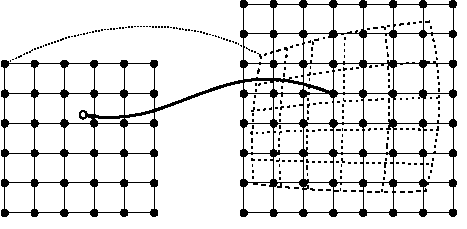
\includegraphics[scale=1.0]{06_bodoveoperace/images/img_6_8.pdf}
    \end{center}
    \caption{Nelineární geometrická transformace.}
    \label{img:6_8}
\end{figure}

Je zřejmé, že čím je požadovaná geometrická transformace komplikovanější, tím vyšší stupeň polynomů je nutné v~rovnicích \eqref{eq:6_28}, \eqref{eq:6_29} zvolit. Jestliže by stupeň polynomů přesáhl rozumnou mez (řekněme např. 3 až 5), pak je lepší použít postupu, kdy vstupní i výstupní obraz rozdělíme na oblasti a transformační polynomy stanovíme zvlášť pro každou dílčí oblast. Stupeň polynomů může být v~tomto případě nízký, protože s~ohledem na složitost transformace můžeme volit jemnost dělení. Nejčastěji se proto v~tomto případě používají polynomy bilineární. Transformaci využívající dělení na podoblasti lze zadat tak, že výstupní  obraz pokryjeme čtyřúhelníkovou sítí a ve vstupním obraze definujeme odpovídající síť transformovanou (obr. \ref{img:6_9}). Síť zadáváme polohou uzlových kontrolních bodů ve vstupním i výstupním obraze. Nejsnáze se implementuje případ, kdy je síť ve výstupním obraze obdélníková. Při praktické realizaci transformace se opět probírají všechny body výstupního obrazu. Podle toho, do které oblasti výstupního obrazu bod padl, se použije odpovídající transformační vztah. Pro \textit{i}-tou oblast má vztah tvar 

\begin{equation} \label{eq:6_31}
    \varphi _{i} \left(x,y\right)=x+\left(a_{i} x+b_{i} y+c_{i} xy+d_{i} \right),
\end{equation}

\begin{equation} \label{eq:6_32}
    \psi_{i} \left(x,y\right)=y+\left(e_{i} x+f_{i} y+g_{i} xy+h_{i} \right).
\end{equation}

\begin{figure}[th]
    \begin{center}
        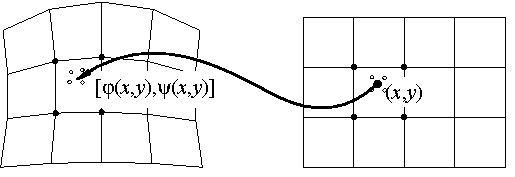
\includegraphics[scale=1.0]{06_bodoveoperace/images/img_6_9.pdf}
    \end{center}
    \caption{Geometrická transformace s rozdělením obrazu na oblasti.}
    \label{img:6_9}
\end{figure}

Neznámé hodnoty \textit{a}$_i$,\textit{b}$_i$,\textit{c}$_i$,\textit{d}$_i$,\textit{e}$_i$,\textit{f}$_i$,\textit{g}$_i$,\textit{h}$_i$ určíme pro každou oblast z~podmínky, aby se vrcholy oblasti (uzlové kontrolní body) transformovaly tak, jak bylo předepsáno. Pro každou oblast máme čtyři vrcholy po dvou souřadnicích, což dává celkem osm rovnic potřebných pro určení hledaných hodnot.

Pro nelineární geometrické operace bývá někdy používáno termínu warping (borcení, kroucení). V televizní tvorbě se v poslední době stala populární také technika nazývaná morphing, která provádí plynulou změnu jednoho objektu v jiný. Předpokládejme, že je zadán počáteční a cílový obraz (označme je \textit{f}$_\mathrm{s}$(\textit{x},\textit{y}), \textit{f}$_\mathrm{d}$(\textit{x},\textit{y})). Úkolem je vytvořit sekvenci \textit{f}$_i$(\textit{x},\textit{y}) obrazů zachycující postupnou změnu obrazu počátečního v cílový. Jistou možností řešení zadaného úkolu by bylo použít prolínání obrazů podle jednoduchého předpisu

\begin{equation} \label{eq:6_33}
    f_{i} \left(x,y\right)=\left(1-\lambda \right)f_\mathrm{s} \left(x,y\right)+\lambda f_\mathrm{d} \left(x,y\right)
\end{equation}
při hodnotě $\lambda$ postupně se zvyšující od 0 do 1. Výsledky samotného prolínání však zpravidla nejsou přesvědčivé. Lepšího dojmu lze dosáhnout kombinací prolínání s nelineární geometrickou transformací. K definování transformace lze použít sítě kontrolních bodů, kterou pokryjeme počáteční i cílový obraz. Polohu kontrolních bodů předepíšeme tak, aby bylo dosaženo požadované deformace obrazu (obr. \ref{img:6_10}). Sítí je nutné pokrýt i obrazy mezilehlé, v nichž lze však síť generovat automaticky pomocí interpolace. Ke generování \textit{i}-tého mezilehlého obrazu použijeme vztahu

\begin{equation} \label{eq:6_34}
    f_i (x, y) = (1 - \lambda) f_\mathrm{s} \left[ \varphi_{i, \mathrm{s}}(x, y), \psi_{i, \mathrm{s}} (x, y) \right] + \lambda f_\mathrm{d} \left[ \varphi_{i, \mathrm{d}} (x, y), \psi_{i, \mathrm{d}} (x,y) \right],
\end{equation}
kde $\varphi_{i, \mathrm{s}}$, $\psi_{i, \mathrm{s}}$, $\varphi_{i, \mathrm{d}}$, $\psi_{i, \mathrm{d}}$ jsou po částech bilineární funkce transformující souřadnice z \textit{i}-tého mezilehlého obrazu do obrazu počátečního resp. cílového. Uvedené funkce jsou určeny zadanou sítí.

\begin{figure}[th]
    \begin{center}
        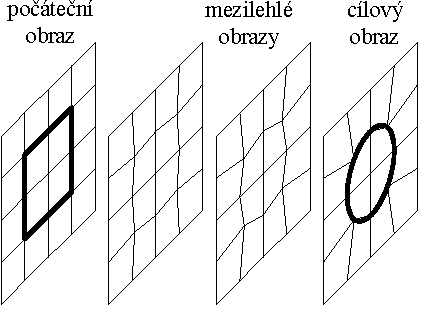
\includegraphics[scale=1.0]{06_bodoveoperace/images/img_6_10.pdf}
    \end{center}
    \caption{Proměna čtverce na kružnici pomocí morphingu.}
    \label{img:6_10}
\end{figure}

